% Name: Higgs production by gluon fusion
% Description: Two gluons fuse through a top-quark loop into a Higgs boson, the main way the Higgs is made at the LHC.
% Tags: Higgs boson, gluon fusion, top quark, loop

\usepackage[compat=1.1.0]{tikz-feynman}

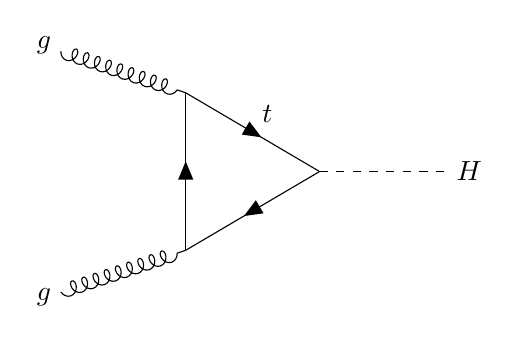
\begin{tikzpicture}
  \begin{feynman}
    \vertex (a) at (0,1);
    \vertex (b) at (0,-1);
    \vertex (c) at (1.7,0);
    \vertex (g1) at (-1.8,1.6) {$g$};
    \vertex (g2) at (-1.8,-1.6) {$g$};
    \vertex (h) at (3.6,0) {$H$};
    \diagram* {
      (g1) -- [gluon] (a),
      (g2) -- [gluon] (b),
      (a) -- [fermion, edge label=$t$] (c) -- [fermion] (b) -- [fermion] (a),
      (c) -- [scalar] (h),
    };
  \end{feynman}
\end{tikzpicture}
